\chapter{Experiments} \label{ch:experiments}
This chapter presents the empirical results of all experimental configurations evaluated across the cohort of 36 patients. Section~\ref{sec:exp:baseline} establishes the baseline performance. Sections~\ref{sec:exp:obj1} through~\ref{sec:exp:obj3} detail the results for each specific research objective. Section~\ref{sec:exp:overall} concludes with a comprehensive comparative summary.

% ================================================================
\section{Baseline: Single-Step Forecasting} \label{sec:exp:baseline}
% ================================================================
\begin{planned}
    \item Reporting of the baseline results under mean squared error optimization, including Mean~Lag to quantify the systematic temporal misalignment.
    \item Include a plot showing a single-patient trajectory comparison to visually demonstrate the systematic prediction delay.
    \item Include the population-level histogram of the per-patient best-lag to prove the time shift is systematic across the cohort.
\end{planned}

\begin{table}[htbp]
\centering
\caption{Baseline single-step forecasting performance under standard MSE training. Mean~Lag is the average absolute shift in minutes that minimises per-patient RMSE ($|\Delta^*| \times 5$~min). RMSE and MAE are in mg/dL; Hypo-F1 is derived by thresholding each 60-min prediction at 70~mg/dL. Means over 36 patients.}
\label{tab:exp:baseline}
\begin{tabular}{lrrrr}
\toprule
Model & RMSE\,$\downarrow$ & Mean~Lag\,$\downarrow$ (min) & MAE\,$\downarrow$ & Hypo-F1\,$\uparrow$ \\
\midrule
LSTM\,MSE      & 36.09 & 51.2 & 27.12 & 0.005 \\
PatchTST\,MSE  & 39.27 & 55.3 & 29.00 & 0.061 \\
\bottomrule
\end{tabular}
\end{table}

\begin{figure}[htbp]
    \centering
    
\includegraphics[width=0.9\textwidth]{patient_85202.png}
    \caption[60min predictions comparison]{Baseline forecasting trajectories for patient 85202 (the Optuna tuning patient). The selected window contains a hypoglycaemia episode (glucose below 70~mg/dL). Both the LSTM and PatchTST predictions follow the glucose shape closely but arrive approximately 55 to 60~minutes late, so the predicted threshold crossing occurs after the true event.}
    \label{fig:exp:baseline_curves}
\end{figure}

\begin{figure}[htbp]
    \centering
    
\includegraphics[width=\textwidth]{lag_distribution.png}
    \caption{Distribution of the per-patient optimal alignment shift $\Delta^*$ across the cohort for LSTM (left) and PatchTST (right) baseline models. $\Delta^*$ is the integer shift in 5-min steps that minimises the RMSE between the shifted prediction and the ground truth. Nearly all patients cluster near the full 60-min forecast horizon, confirming that the temporal misalignment is a systematic, cohort-wide phenomenon.}
    \label{fig:exp:lag_dist}
\end{figure}


% ================================================================
\section{Objective 1: Offset-Aware Loss Functions} \label{sec:exp:obj1}
% ================================================================
\subsection{Bounded-Lag Loss Results}
\begin{planned}
    \item Description of the results when optimizing with a predefined local neighborhood.
    \item Statistical reporting of the marginal gains in event-centric detection performance.
\end{planned}

\subsection{Soft-DTW Loss Results}
\begin{planned}
    \item Detailed analysis of the Soft-DTW optimization outcomes.
    \item Discussion of the expanded temporal alignment variance. Explain why elastic sequence matching during training yields higher residual shape misalignment metrics.
    \item Include a plot comparing standard MSE trajectories against Soft-DTW trajectories to visually explain the trade off between structural shape matching and exact amplitude tracking.
    \item Interpretation of why relaxing temporal constraints fails to supply the structural information needed to anticipate future glycemic changes.
\end{planned}

\begin{table}[htbp]
\centering
\caption{Effect of offset-aware loss functions on forecasting accuracy and mean prediction delay. Mean~Lag is the average absolute shift in minutes that minimises per-patient RMSE ($|\Delta^*| \times 5$~min); lower values indicate predictions are temporally closer to the ground truth. RMSE and MAE are in mg/dL (means over 36 patients).}
\label{tab:exp:obj1}
\begin{tabular}{llrrrr}
\toprule
Architecture & Loss & RMSE\,$\downarrow$ & Mean~Lag\,$\downarrow$ (min) & MAE\,$\downarrow$ & Hypo-F1\,$\uparrow$ \\
\midrule
\multicolumn{6}{l}{\textit{LSTM}} \\[2pt]
 & MSE (baseline) & 36.09 & 51.2          & 27.12 & 0.005 \\
 & Bounded-Lag    & 36.14 & 48.6          & 27.57 & 0.014 \\
 & Soft-DTW       & 37.23 & \textbf{46.0} & 28.76 & 0.014 \\
\midrule
\multicolumn{6}{l}{\textit{PatchTST}} \\[2pt]
 & MSE (baseline) & 39.27 & 55.3          & 29.00 & 0.061 \\
 & Bounded-Lag    & 39.30 & 54.6          & 29.03 & 0.067 \\
 & Soft-DTW       & 43.24 & 54.4          & 32.25 & 0.062 \\
\bottomrule
\end{tabular}
\end{table}

\begin{figure}[htbp]
    \centering
    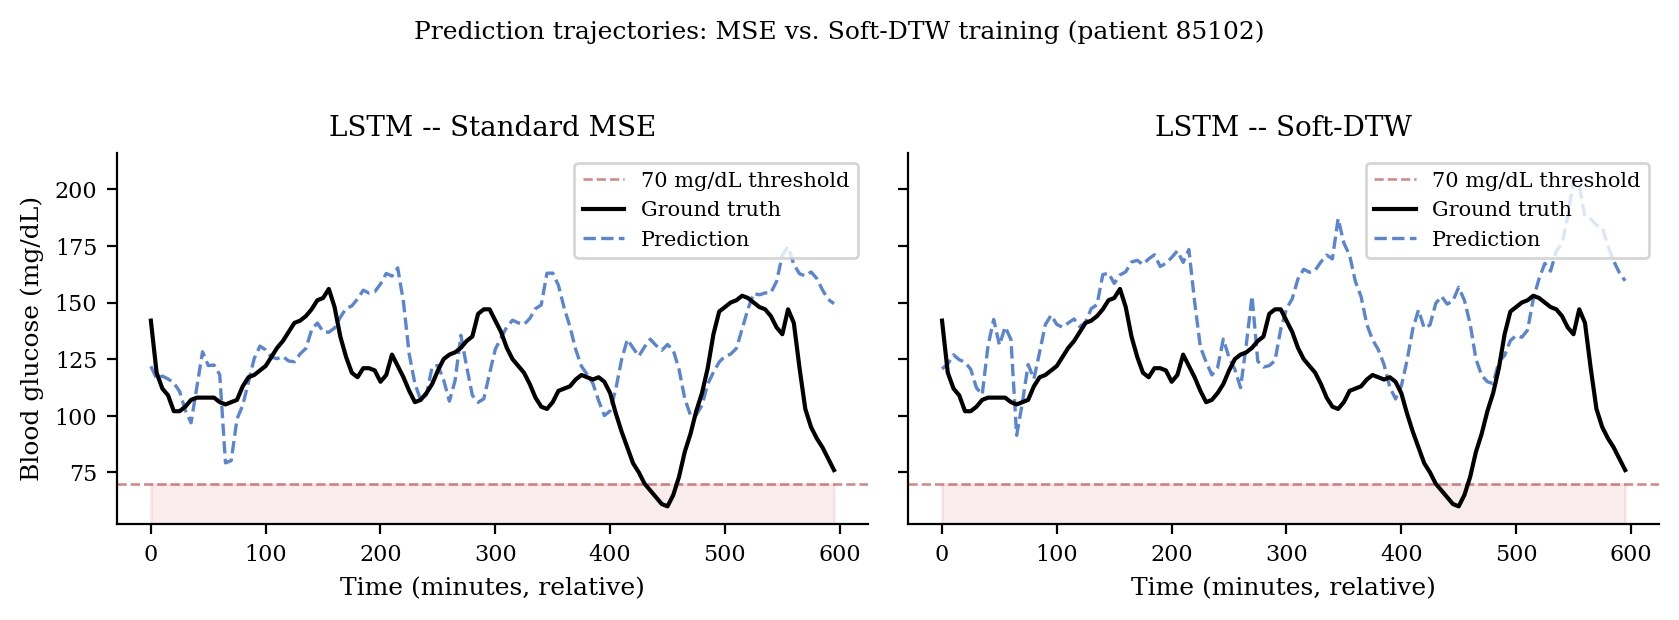
\includegraphics[width=\textwidth]{dtw_vs_mse_trace.png}
    \caption{Prediction trajectories for a representative patient window (patient 85102, 10-hour window) under standard MSE training (left) and Soft-DTW training (right). Both models exhibit a temporal lag of comparable magnitude and neither eliminates the systematic phase offset. The Soft-DTW prediction shows marginally higher amplitude variance consistent with the elastic shape-matching objective, at the cost of a higher RMSE (Table~\ref{tab:exp:obj1}).}
    \label{fig:exp:soft_dtw_plot}
\end{figure}


% ================================================================
\section{Objective 2: Multi-Step Forecasting} \label{sec:exp:obj2}
% ================================================================
\begin{planned}
    \item Reporting of the direct multi-step sequence supervision results.
    \item Interpretation of how simultaneous loss minimization across early steps acts as a temporal anchor to maintain phase coherence.
    \item Include a plot demonstrating the improved phase alignment of the multi-step approach compared to the single-step baseline.
\end{planned}

\begin{table}[htbp]
\centering
\caption{Effect of multi-step sequence supervision on forecasting accuracy and mean prediction delay. Multi-step supervision reduces the mean lag for both architectures. RMSE and MAE are in mg/dL (means over 36 patients).}
\label{tab:exp:obj2}
\begin{tabular}{llrrr}
\toprule
Architecture & Supervision & RMSE\,$\downarrow$ & Mean~Lag\,$\downarrow$ (min) & MAE\,$\downarrow$ \\
\midrule
\multicolumn{5}{l}{\textit{LSTM}} \\[2pt]
 & Single-step (baseline) & 36.09 & 51.2                  & 27.12 \\
 & Multi-step             & 35.59 & \textbf{50.1}         & 26.80 \\
\midrule
\multicolumn{5}{l}{\textit{PatchTST}} \\[2pt]
 & Single-step (baseline) & 39.27 & 55.3                  & 29.00 \\
 & Multi-step             & 39.05 & 54.6                  & 28.84 \\
\bottomrule
\end{tabular}
\end{table}

\begin{figure}[htbp]
    \centering
    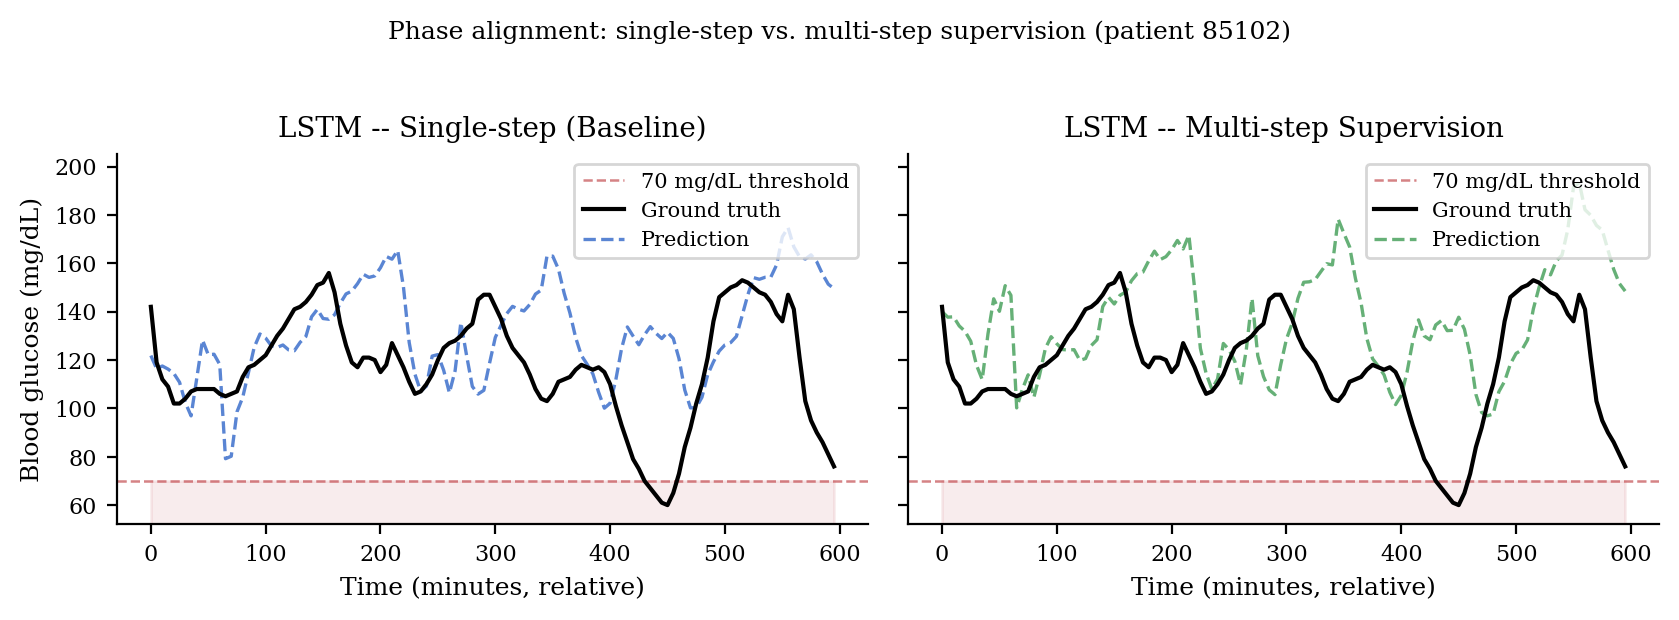
\includegraphics[width=\textwidth]{multistep_vs_baseline_trace.png}
    \caption{Prediction trajectories for a representative patient window (patient 85102) under single-step baseline training (left) and multi-step sequence supervision (right). A hypoglycaemia episode is visible in the ground truth near the end of the window. The multi-step model exhibits marginally improved phase coherence, consistent with the Lag-RMSE reduction reported in Table~\ref{tab:exp:obj2}.}
    \label{fig:exp:multistep_plot}
\end{figure}


% ================================================================
\section{Objective 3: Event-Centric Evaluation} \label{sec:exp:obj3}
% ================================================================
\begin{planned}
    \item Evaluation of the forecast-derived event detectors across tolerance ranges.
    \item Include the $\tau$-Sweep plot to visually track F1 curves across tolerance ranges. Interpret the flat response as empirical evidence of the static prediction delay.
    \item Reporting of the direct binary event classifier performance.
    \item Include a plot showing the direct classifier output trace (probabilities vs.\ true events) to highlight the performance inversion between the recurrent model and the instance-normalized transformer.
\end{planned}

\begin{table}[htbp]
\centering
\caption{Comprehensive summary of all eight training configurations. Bold values mark the best result per column. Mean~Lag is the average absolute shift in minutes that minimises per-patient RMSE ($|\Delta^*| \times 5$~min). RMSE and MAE are in mg/dL; Hypo-F1 is derived from threshold-based event detection at 70~mg/dL. For detailed event-detector confusion counts see Fig.~\ref{fig:app:confusion_counts}.}
\label{tab:exp:overall}
\begin{tabular}{llrrrr}
\toprule
Architecture & Training & RMSE\,$\downarrow$ & Mean~Lag\,$\downarrow$ (min) & MAE\,$\downarrow$ & Hypo-F1\,$\uparrow$ \\
\midrule
\multicolumn{6}{l}{\textit{LSTM}} \\[2pt]
 & MSE (baseline) & 36.09 & 51.2                  & 27.12          & 0.005 \\
 & Bounded-Lag    & 36.14 & 48.6                  & 27.57          & 0.014 \\
 & Soft-DTW       & 37.23 & \textbf{46.0}         & 28.76          & 0.014 \\
 & Multi-step     & \textbf{35.59} & 50.1         & \textbf{26.80} & 0.010 \\
\midrule
\multicolumn{6}{l}{\textit{PatchTST}} \\[2pt]
 & MSE (baseline) & 39.27 & 55.3                  & 29.00          & 0.061 \\
 & Bounded-Lag    & 39.30 & 54.6                  & 29.03          & 0.067 \\
 & Soft-DTW       & 43.24 & 54.4                  & 32.25          & 0.062 \\
 & Multi-step     & 39.05 & 54.6                  & 28.84          & \textbf{0.072} \\
\bottomrule
\end{tabular}
\end{table}

\begin{figure}[htbp]
    \centering
    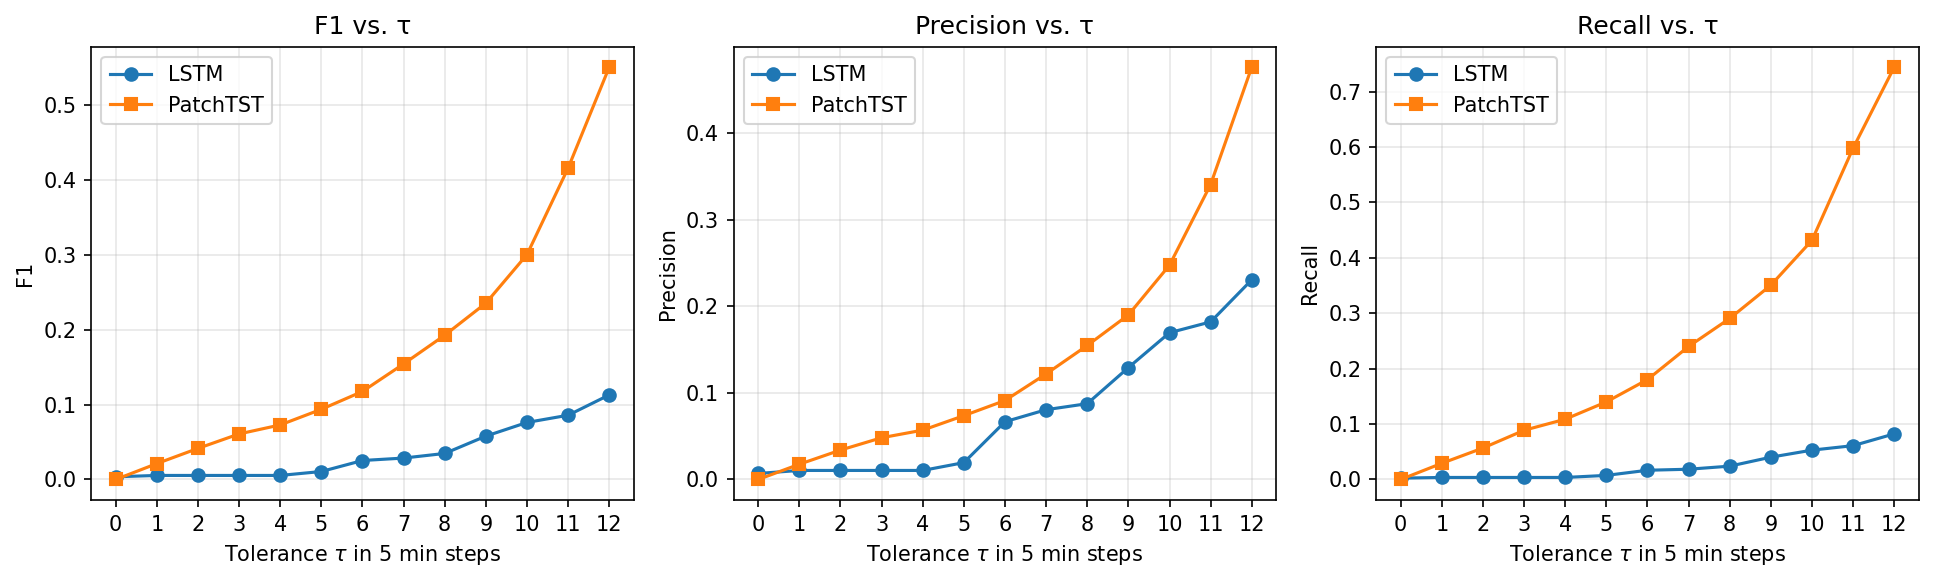
\includegraphics[width=\textwidth]{tau_sweep_comparison.png}
    \caption{Forecast-derived hypoglycaemia detection performance (F1, Precision, Recall) as a function of the tolerance window $\tau$ for the LSTM and PatchTST MSE baselines. All three metrics increase monotonically with $\tau$, confirming that the improvement comes from accepting delayed detections rather than from genuine anticipatory prediction.}
    \label{fig:exp:tau_sweep_plot}
\end{figure}

\begin{table}[htbp]
\centering
\caption{Event detection performance (Task~A: ``will a hypoglycaemia event occur anywhere in the next 60~min?''). F2 weights recall twice as heavily as precision, reflecting the clinical priority of minimising missed events. The Naive Last Value baseline fires only when glucose is already below 70~mg/dL. The forecast-derived entry uses threshold crossing of the 60-min Soft-DTW PatchTST prediction.}
\label{tab:exp:classifiers}
\begin{tabular}{lrrrr}
\toprule
Model & Precision\,$\uparrow$ & Recall\,$\uparrow$ & F1\,$\uparrow$ & F2\,$\uparrow$ \\
\midrule
\multicolumn{5}{l}{\textit{Rule-based baselines}} \\[2pt]
 Naive last value               & 0.857 & 0.326 & 0.473 & 0.373 \\
 Naive mean                     & 0.396 & 0.041 & 0.074 & 0.050 \\
\midrule
\multicolumn{5}{l}{\textit{Forecast-derived detector}} \\[2pt]
 PatchTST Soft-DTW (threshold)  & 0.056 & 0.129 & 0.062 & 0.103 \\
\midrule
\multicolumn{5}{l}{\textit{Trained direct classifiers}} \\[2pt]
 LSTM event classifier          & 0.237 & \textbf{0.693} & 0.334 & \textbf{0.463} \\
 PatchTST event classifier      & 0.054 & 0.615          & 0.095 & 0.179          \\
\bottomrule
\end{tabular}
\end{table}

\begin{figure}[htbp]
    \centering
    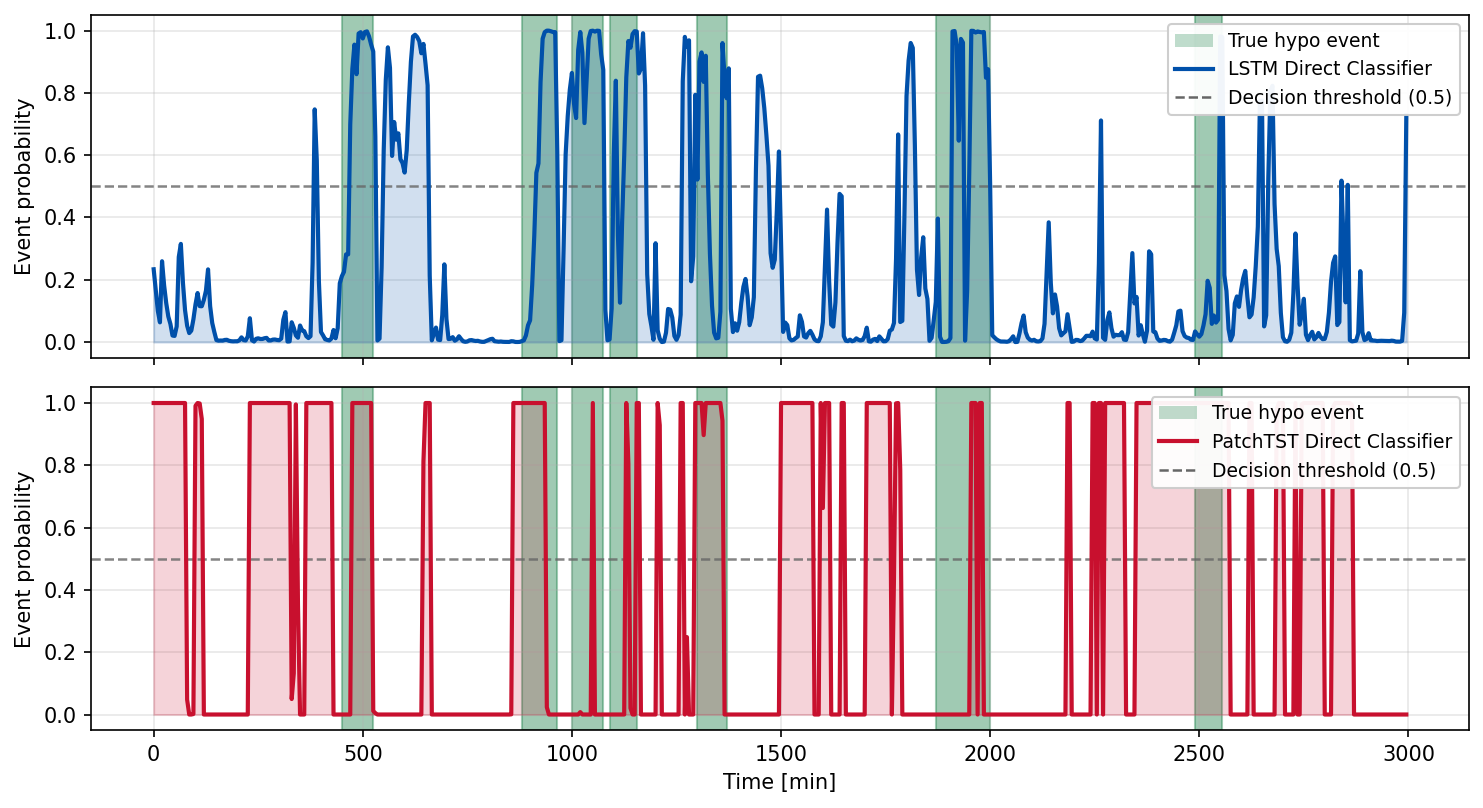
\includegraphics[width=0.9\textwidth]{classifier_predictions.png}
    \caption{Output traces of the LSTM (top) and PatchTST (bottom) direct event classifiers for a representative patient segment. The LSTM produces focused, high-confidence alarms; the PatchTST fires persistently across the window, yielding substantially higher recall at the cost of far more false positives. The absolute counts across the full cohort are shown in Fig.~\ref{fig:app:confusion_counts}.}
    \label{fig:exp:classifier_traces}
\end{figure}

\begin{figure}[htbp]
    \centering
    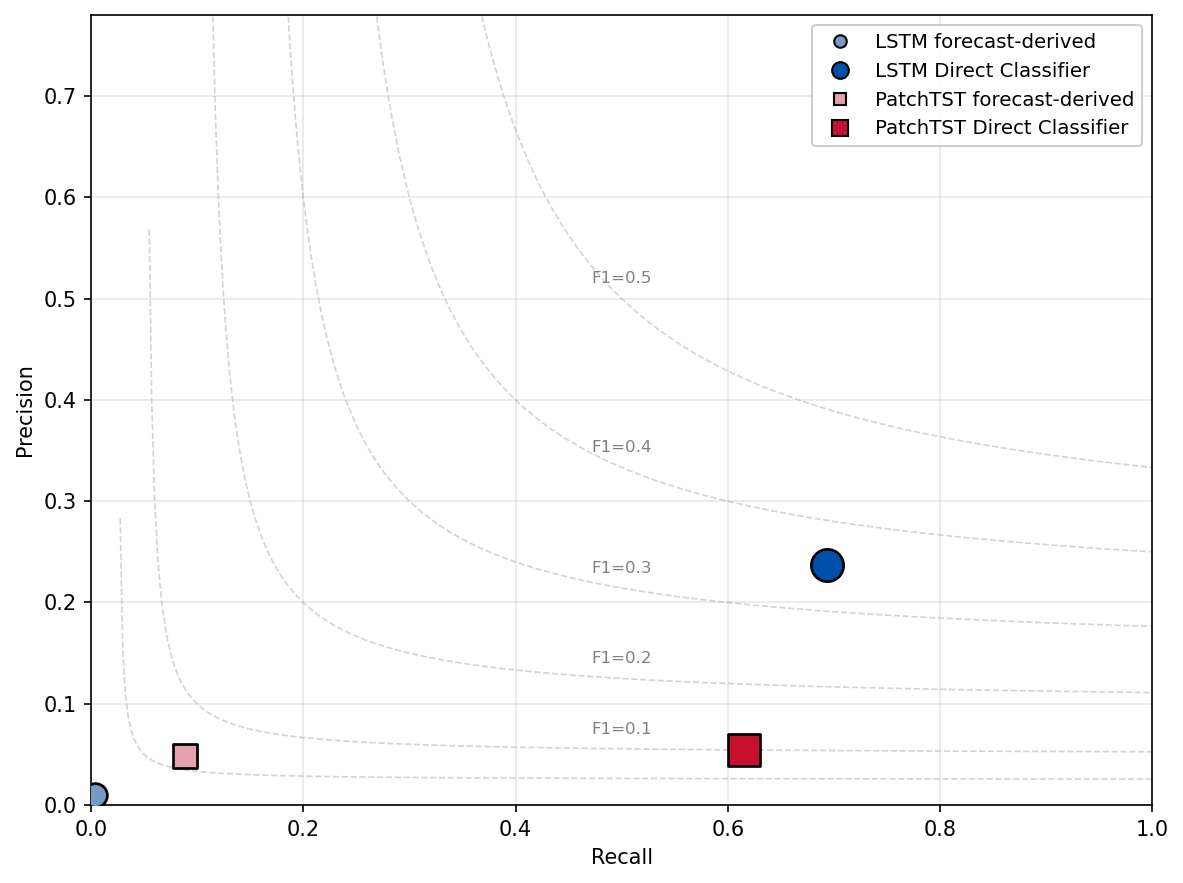
\includegraphics[width=0.9\textwidth]{pr_paradox.png}
    \caption{Precision--Recall space for forecast-derived detectors (hollow markers) and direct binary classifiers (filled markers) for LSTM (circles) and PatchTST (squares). The forecast-derived detectors cluster near the origin due to the systematic prediction delay. Direct training on the classification task dramatically shifts both models into clinically relevant recall regimes, with the LSTM achieving the superior precision--recall trade-off.}
    \label{fig:exp:pr_paradox}
\end{figure}

\begin{figure}[htbp]
    \centering
    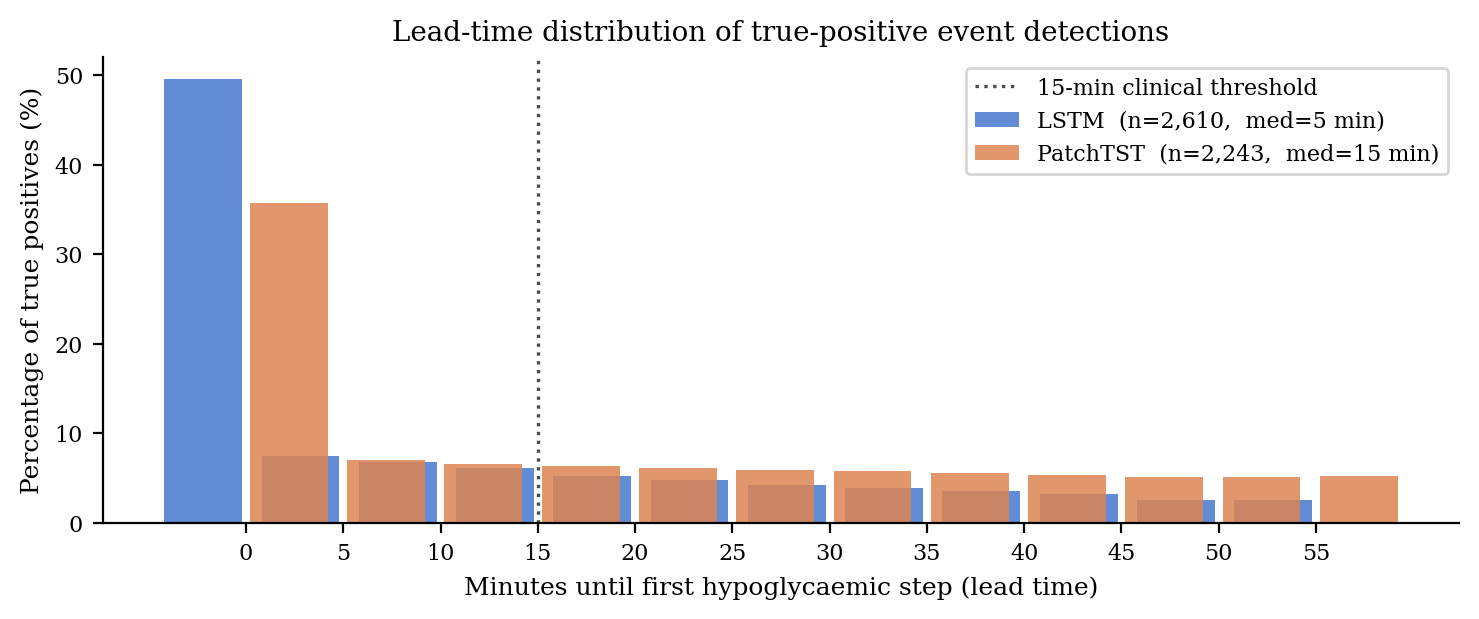
\includegraphics[width=0.9\textwidth]{lead_time_distribution.png}
    \caption{Distribution of lead times for true-positive detections by the LSTM and PatchTST direct event classifiers. Lead time is the elapsed time in minutes from alarm issuance to the first hypoglycaemic step in the prediction window. For the LSTM, 49.5\% of true positives carry a lead time of 0~min, meaning the hypoglycaemic event is already in progress at the moment of detection. The PatchTST shows a more evenly distributed lead time with a median of 15~min, at the cost of substantially more false alarms (Table~\ref{tab:exp:classifiers}).}
    \label{fig:exp:lead_time}
\end{figure}


% ================================================================
\section{Overall Comparison} \label{sec:exp:overall}
% ================================================================
\begin{planned}
    \item Descriptive summary of the global metrics across all tested configurations (see Table~\ref{tab:exp:overall} above).
    \item Final structural recommendation motivating a decoupled dual-model system.
\end{planned}
